\documentclass[conference]{IEEEtran}
\IEEEoverridecommandlockouts
%The preceding line is only needed to identify funding in the first footnote. If that is unneeded, please comment it out.


%\usepackage{cite}
\usepackage{amsmath,amssymb,amsfonts}
\usepackage{algorithmic}
\usepackage{graphicx}
\usepackage{textcomp}
\usepackage{xcolor}

% JH/zusätzliche Packages, die ich verwendet habe
\usepackage{hyperref}


% JH/Definition eigener Befehle
\newcommand{\R}{\mathbb{R}}
\newcommand{\N}{\mathbb{N}}
\newcommand{\TSShoch}{\mathhbb\textsuperscript{}}
%\textsuperscript{2}

\def\BibTeX{{\rm B\kern-.05em{\sc i\kern-.025em b}\kern-.08em
    T\kern-.1667em\lower.7ex\hbox{E}\kern-.125emX}}
    
    
\usepackage[backend=bibtex, style=numeric]  
           {biblatex}
\addbibresource{Literature.bib}   
    
\begin{document}

\title{Diode pumped $Pr^{3+}$:LiYF4 lasers emitting at 640 nm, 604 nm and 523 nm\\
}

\author{Niklas H.}

\maketitle

\begin{abstract}
In this report, a Praseodymium doped LiYF4 (Pr:YLF) laser consisting of a hemispheric cavity of 50 mm (640 nm) or 100 mm (604nm/523nm) and a 6mm long longitudinally pumped crystal (0.8 at\% doping) is reported. Depending on the mirror set used, the 640 nm ($^3P_0$ to $^3F_2$), 607 nm ($^3P_0$ to $^3H_6$) and 523 nm ($^3P_0$ to $^3H_5$) lines of the $Pr^{3+}$-Ion can be amplified. Slope effiencies of 28.4\%, 5.6\% and 2.5\% respectively were reached with maximum output powers of 149 mW, 26 mW  and 4.3 mW.
\end{abstract}

\begin{IEEEkeywords}
LiYF4 Laser, DPSS Laser, Pr:YLF Laser
\end{IEEEkeywords}
%-------------------------------------------------------------------------------------
\section{Introduction}
%-------------------------------------------------------------------------------------

Since the introduction of lasers in 1960 by Theodore Maiman, many gain media for obtaining optical gain and therefore laser action have been introduced. One of these media is LiYF4 doped with $Pr^{3+}$-Ions (Pr:YLF), which is able to operate at multiple lines, e.g. 720nm, 607nm, 640nm and 523nm, which is why special research efforts have been directed towards this material. It is also one of the few gain media which directly (without frequency doubling) emit visible light and also are pumped by visible light. Furthermore, continous wave UV emission by intracavity doubling has been reported \cite{Richter.2006}\cite{Gun.2011}. For this report, the 640 nm ($^3P_0$ to $^3F_2$), 607 nm ($^3P_0$ to $^3H_6$) and 523 nm ($^3P_0$ to $^3H_5$) transitions are of relevance. The $Pr^{3+}$-Ion reaches the excited state $^3P_0$ by being excited to the $^3P_2$ state and fastly relaxing to $^3P_0$. The excitation process is performed most efficiently by using 444nm pumplight. Since InGaN laser diodes emit around this exact wavelength and are commercially available at several watts of optical power, they have been used extensively for pumping Pr:YLF lasers \cite{Xu.2013}\cite{Krankel.2016}\cite{Bellancourt.2010}\cite{Luo.2018}\cite{Muller.2011}. For linear end-pumped resonator designs using InGaN laser diodes, slope efficiencies of 49\% for 523 nm, 40\% at 607 nm and 57\% for 640 nm have been reported \cite{Luo.2016}. 
\section{Experimental setup}
The resonator setups for amplifying the 607 nm and 640 nm lines are a standard hemispherical cavity with the concave outcoupling mirror as reported in e.g. \cite{Luo.2016} and \cite{Bellancourt.2010}. The setup is depicted in figure \ref{setup607640}.
\begin{figure}[h]
	\centering
	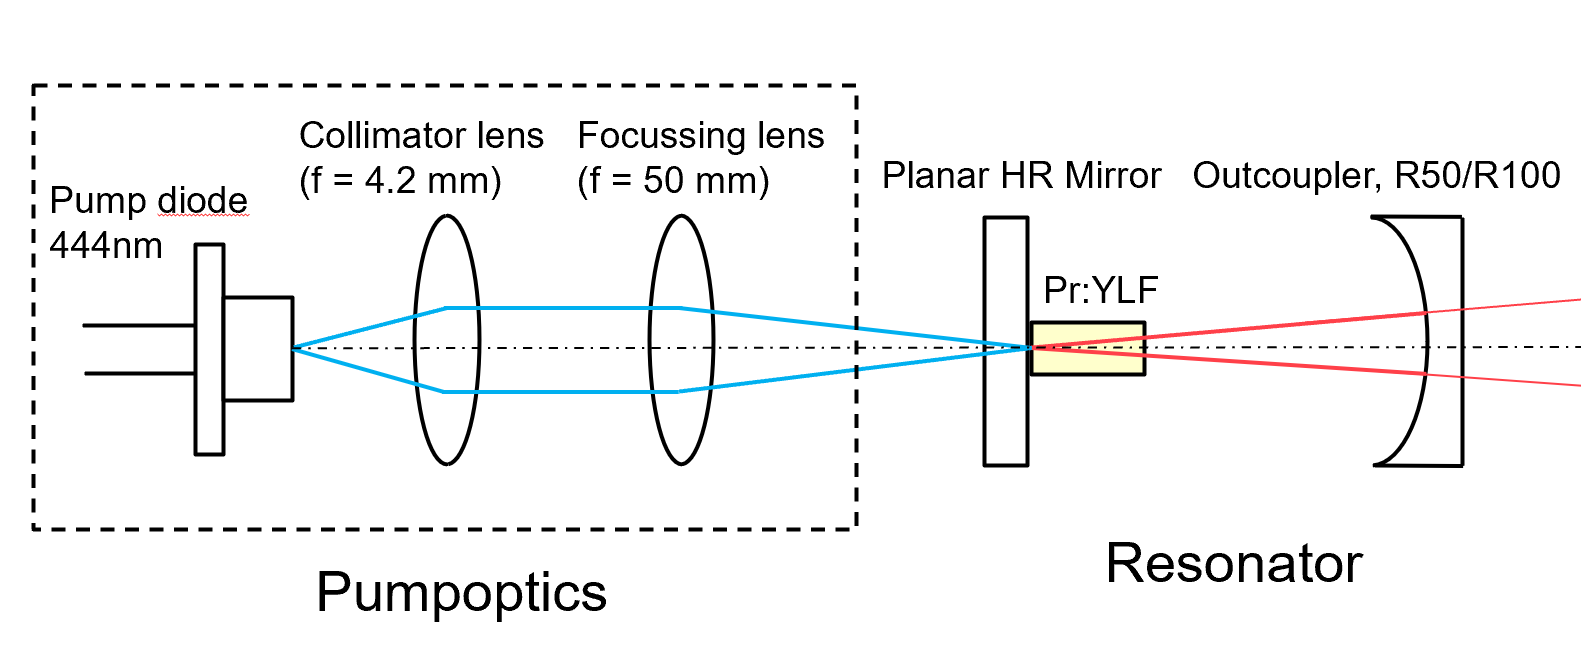
\includegraphics[width=0.4\textwidth]{img/setup607640}
	\caption{Setup for 607 nm and 640 nm laser output}
	\label{setup607640}
\end{figure}
For 607 nm and 640 nm output couplers (OC) with 1\% T and 1.8\% T are used. The radius of curvature (ROC) and therefore cavity length is 100 mm and 50 mm respectively. The Pr:YLF crystal used has a doping concentration of 0.8 at\% and is 6 mm long. The faces of the crystal are coated with an antireflection coating for 444 nm and 500 nm - 720 nm. It is placed directly in front of the high reflecting mirror (HR), with about 2 mm of air between them. The crystal is glued into an aluminium holder using a thermal glue, in order to passively cool it down. This holder was designed to be water-cooled as well, but this did not prove to be necessary at the power levels produced by the pump diode. A HR with high transmission at 444 nm and high reflectivity at 600 nm - 700 nm are used. The crystal is pumped longitudinally.\\
For pumping, a Nichia NDB7875 laser diode is used. The diode is selected to have an output wavelength of 444 nm at 1.5 A, which corresponds to ~2 W of output power. The pump diode is collimated using an aspheric lens with f = 4.2 mm (Thorlabs A390TM-A) and focussed into the crystal via a bi-convex lens with f = 50 mm (Thorlabs LB1844-A). Both pump optics were delivered with a VIS antireflection coating. The pump diode is water cooled. Since the absorption coefficient of Pr:YLF is highly dependent on polarization \cite{Xu.2013}, the pump diode is rotated until the absorption peaks and then locked rotationally to match the pump polarization and the crystal orientation. \\
Due to availability issues, a different setup for obtaining 523 nm laser output is implemented. This setup is depicted in figure \ref{setup523}.
\begin{figure}[h]
	\centering
	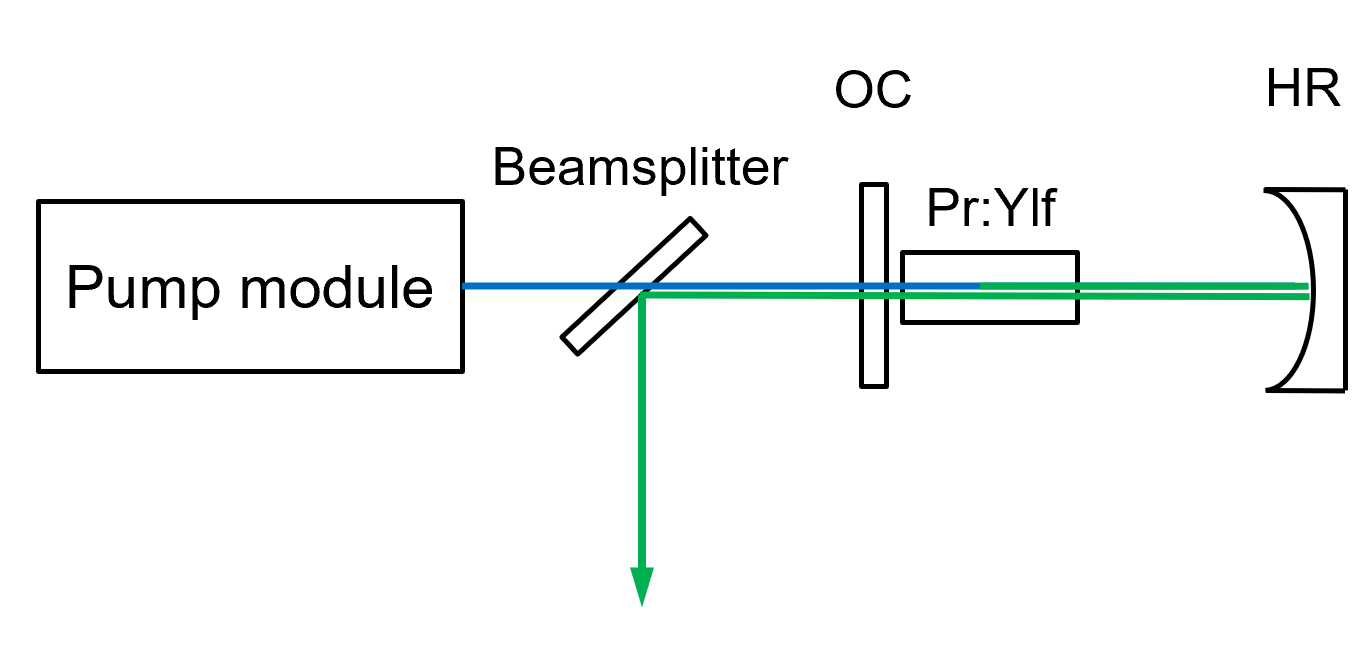
\includegraphics[width=0.4\textwidth]{img/setup523}
	\caption{Setup for 523 nm laser output}
	\label{setup523}
\end{figure}
In this case, the concave mirror is coated with a very high reflective coating ($\geq$ 99.9\% R) for 523 nm. The plane mirror is used as the output coupler, with a transmission of about 0.5\% for 523 nm. A beamsplitter with high transmission for the pumplight and high reflectivity for 523 nm is installed to guide the laser beam out of the setup. 
\section{Results and Discussion}
For measuring the output power of the lasers, each setup is optimized at a set pump power above threshold. Mirror distance and adjustment are fine-tuned for maximum output power. //
The output power of each setup is measured using a photodiode power sensor (Thorlabs S121C with PM100D console). The data can be found in the figures \ref{result640}, \ref{result604} and \ref{result523}.
 \begin{figure}[h]
	\centering
	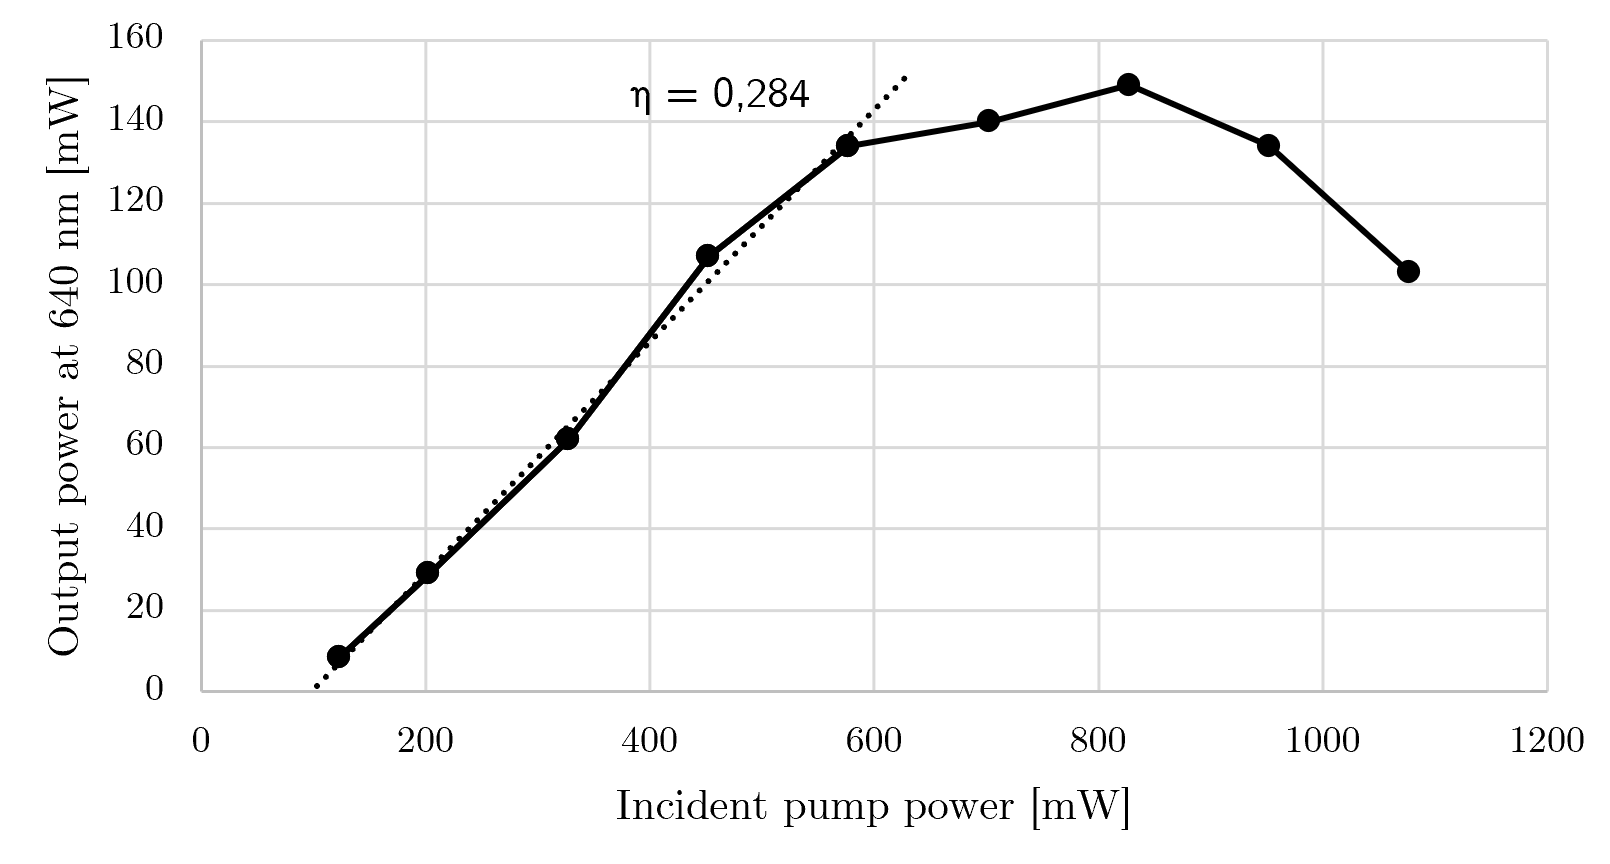
\includegraphics[width=0.4\textwidth]{img/measurement640}
	\caption{Output power at 640 nm over pump power}
	\label{result640}
\end{figure}
 \begin{figure}[h]
	\centering
	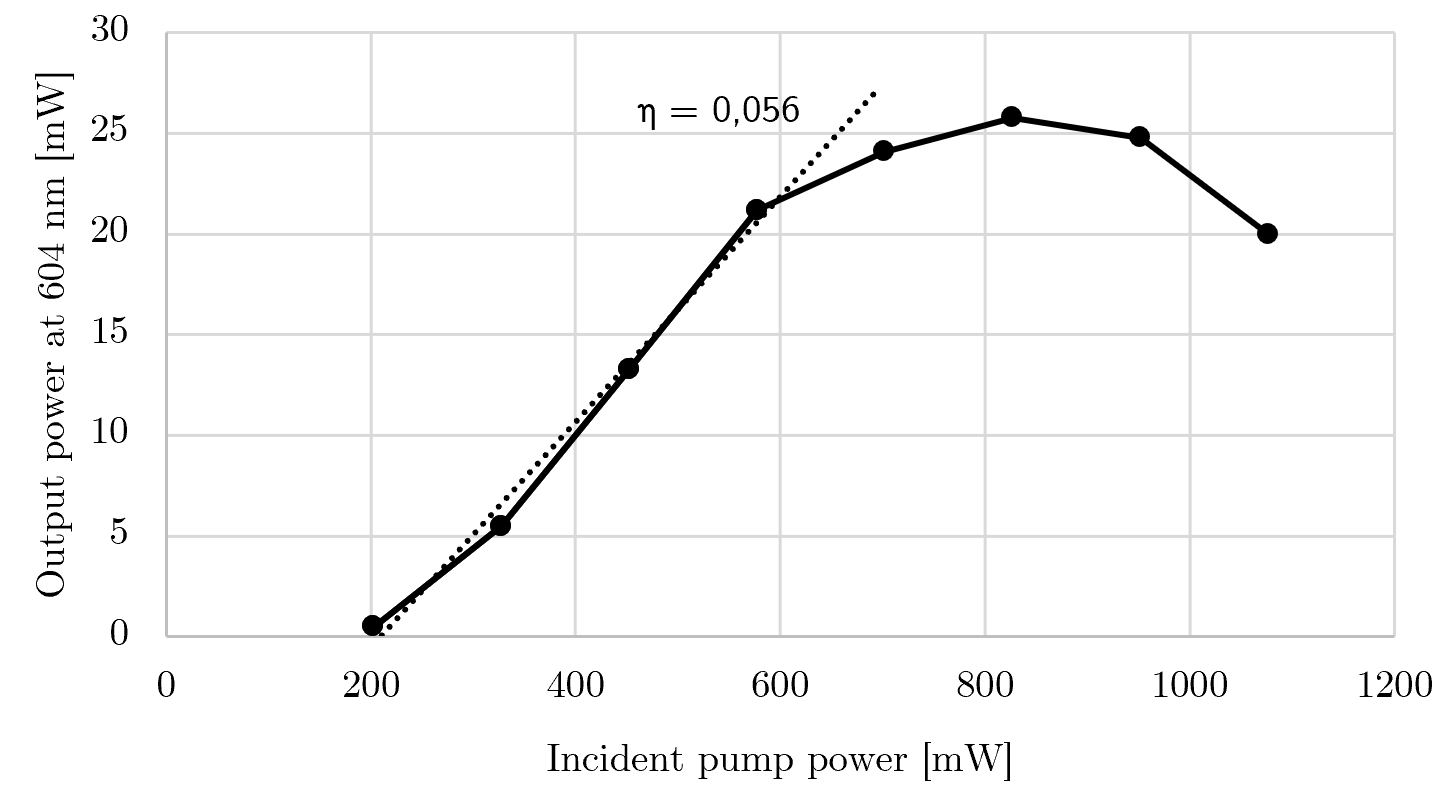
\includegraphics[width=0.4\textwidth]{img/measurement604}
	\caption{Output power at 604 nm over pump power}
	\label{result604}
\end{figure}
For the 640 nm setup, a lasing threshold $P_{th}$ of about 130 mW was achieved. The slope efficiency $\eta_{sl}$ was measured to be 28.4\%. A maximum output power of $P_{max}$ = 149 mW was observed. For the 607 nm, $P_{th}$ was 200 mW, with $\eta_{sl}$ = 5.6\% and $P_{max}$ = 26 mW. Both the higher threshold and lower slope efficiency are to be expected since the emission cross section $\sigma_{em}$ of Pr:YLF at 604 nm is lower than at 640 nm \cite{Richter.2007}. //
The power measurements reveal a rather unusual effect: Both the 604 nm and 640 nm setups scale linearly with the pump powers until about 600 mW of pump power. Beyond 600 mW, the output power starts to saturate and even declines when the pump power is increased more. This effect is pronounced even more in the 523 nm setup (see fig. \ref{result523}). Here, the linear region is relatively small which is due to the higher lasing threshold of 520 mW. This leaves only 100 mW of linear scaling ($\eta_{sl}$ = 2,5\%) until the effect mentioned above sets in at around 650 mW. The much lower slope effiency and $P_{max}$=4,3 mW can again be contributed to lower values for $\sigma_{em}$ at 523 nm  although the difference of $\eta_{sl}$ for 640 nm and 523 nm is much larger than in the literature \cite{Richter.2007}.
\begin{figure}[h]
	\centering
	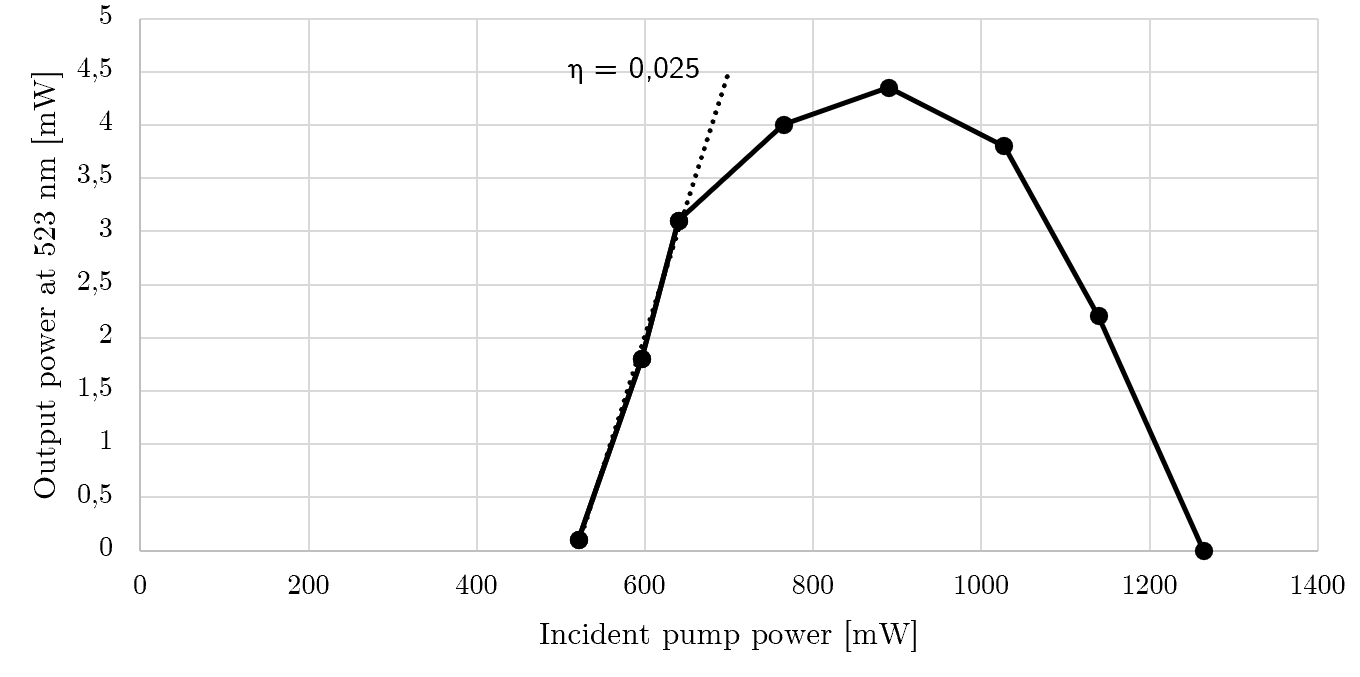
\includegraphics[width=0.4\textwidth]{img/measurement523}
	\caption{Output power at 523 nm over pump power}
	\label{result523}
\end{figure}
It is likely that the power degradation effect is due to power dependencies of the mode structure of the pump diode, which would greatly affect the pump-mode overlap and thus output power. Thermal effects can be ruled out since the effect could be detected across all diode temperatures. Also, current dependent wavelength shifts are unlikely to cause this effect since the laser diode was selected to emit 444 nm at 1500 mA which means that the laser should reach maximum efficiency when approaching this current. Thermal lensing is a possible factor but can not be the main reason since the effect does not creep in slowly whilst the crystal heats up but appears at a very predictable pump power. \\
Due to the lower emission cross sections and thus amplification factors at 523 nm and 604 nm combined with relatively high resonator lengths, both setups are relatively sensitive to misalignments, with the 523 nm setup much more unstable than the 604 nm setup. The 640 nm setup is extraordinarly insensitive to misalignments, resonator lengths of 25 - 50 mm result in reliable laser output, with the power increasing when the resonator length approaches the stability limit at L = 50 mm. The lower misalignment sensitivity is likely due to a smaller mode waist of the shorter resonator and thus higher power density in the pumped region of the crystal and therefore stronger amplification combined with a lower "leverage" \ of the short focal length output coupler. This leads to lower displacements of the mode waist inside the crystal for the same angular movement of the mirror (compared to a longer local length mirror).\\
As mentioned above, the slope effiencies and maximum laser powers achieved in this work are lower than in the reported literature (e.g. \cite{Richter.2007}, \cite{Luo.2016}) which can be attributed to multiple factors. Most importantly, no pump beam shaping techniques besides collimation and focussing where deployed which almost definitely decreases the pump-mode overlap efficiency in the Pr:YLF crystal. Furthermore, the output coupling of the resonators was not optimized. The resonator setups were tuned to local maxima but it is possible that the absolute maximum possible output powers were not reached.
\section{Conclusion}
In this work, setups for amplifying the 523 nm, 604 nm and 640 nm lines of the Pr:YLF crystal were presented and characterized. Slope effiencies of 2.5\%, 5.6\% and 28.4\% respectively were reached with maximum output powers of 4.3 mW, 26 mW and 149 mW. Higher output powers were prevented by a degradation effect starting at around 600 mW of pump power which can likely be attributed to the pump diode. This effect is currently the subject of further examination. Nevertheless, successful lasing was shown for all three setups with the results being in qualitative agreement with the literature.
\section{Acknowledgements}
The author would like to thank the staff of the Institute of Applied Optics and Electronics at the University of Applied Sciences Cologne for providing the opportunity to make laser power measurements in their laboratories.
%-------------------------------------------------------------------------------------
%-------------------------------------------------------------------------------------
%\section*{References}
\printbibliography
%-------------------------------------------------------------------------------------
%-------------------------------------------------------------------------------------
\end{document}
